\subsection{Gradient decent methods}

\begin{figure}[H]
\centering
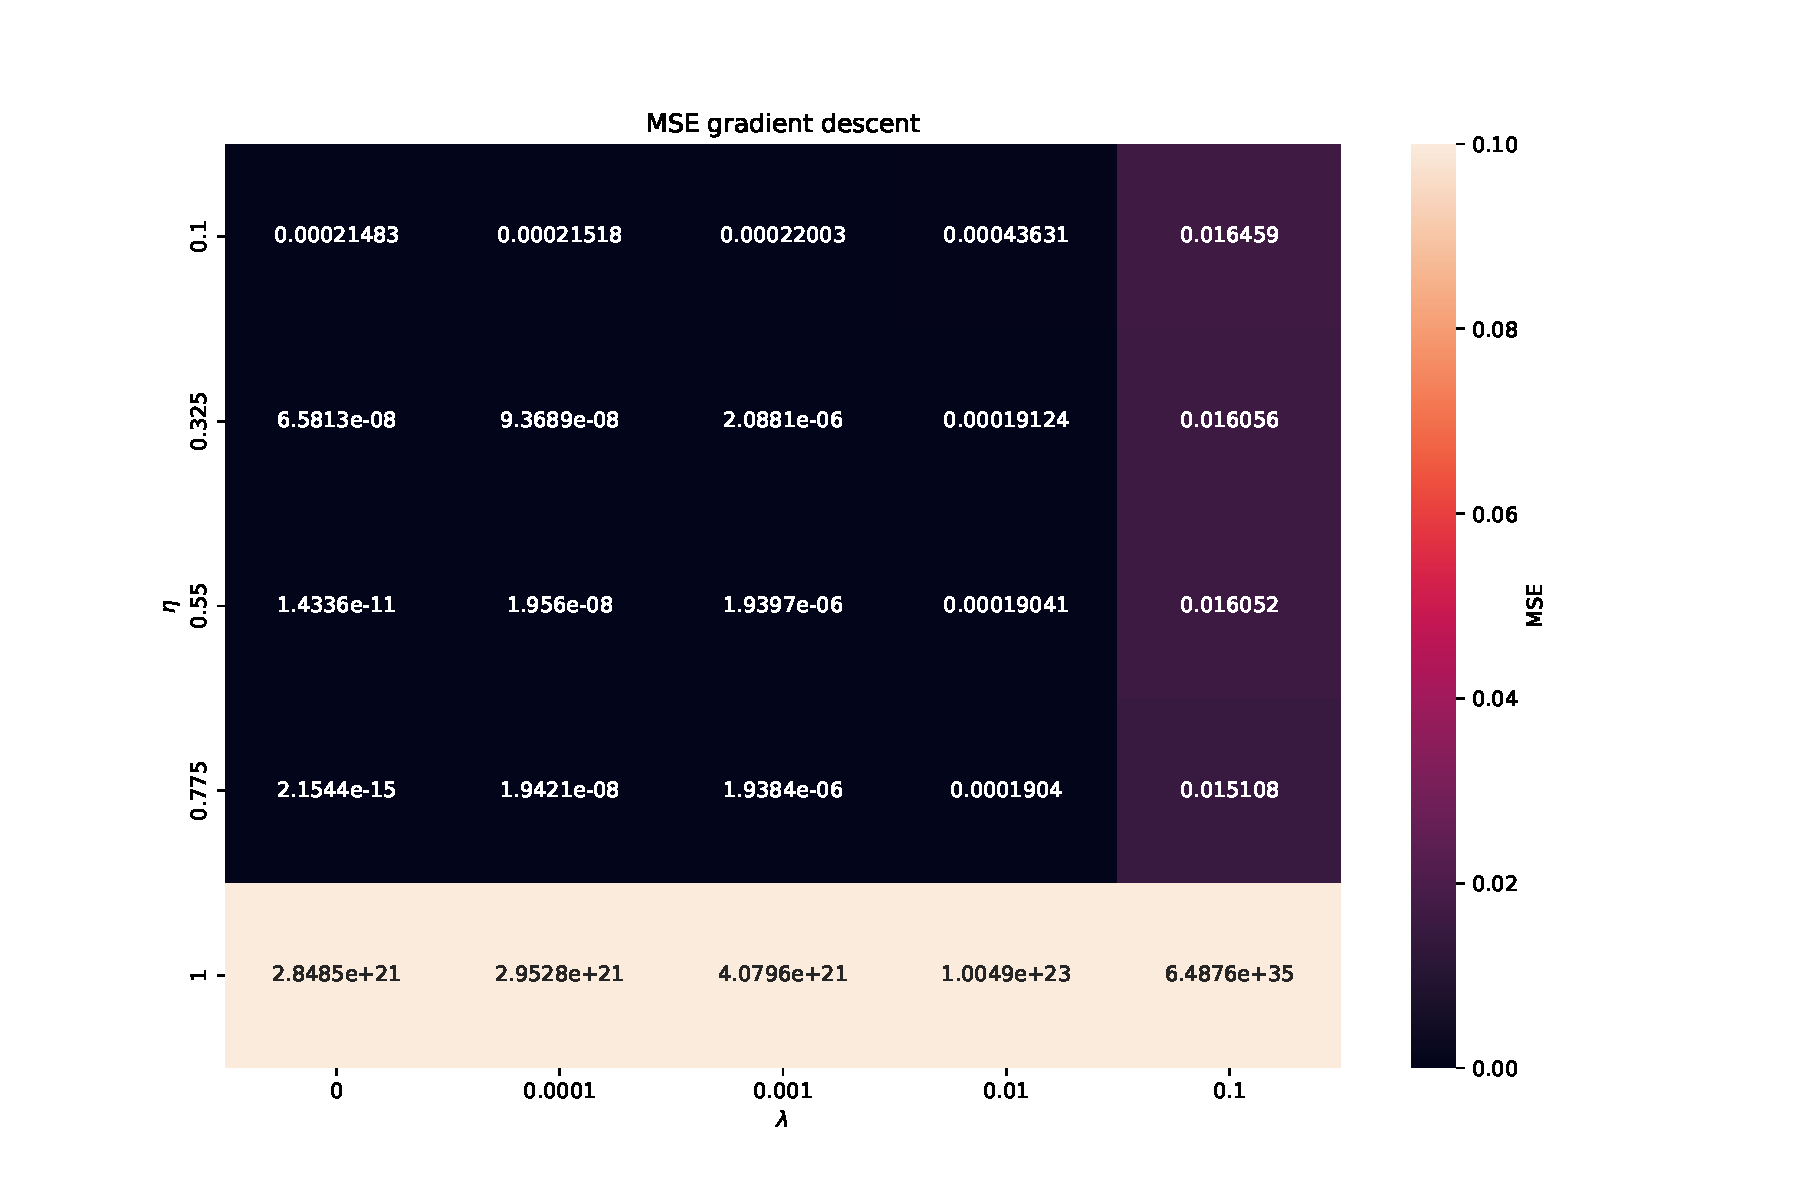
\includegraphics[width=0.8\textwidth]{Figures/PartA/gd_MSE(eta,lmb)}
\caption{Plain gradient descent MSE as a function of \(\eta \) and \(\lambda \).}
\label{fig:gd_MSE-eta-lmb-}
\end{figure}

\begin{figure}[H]
\centering
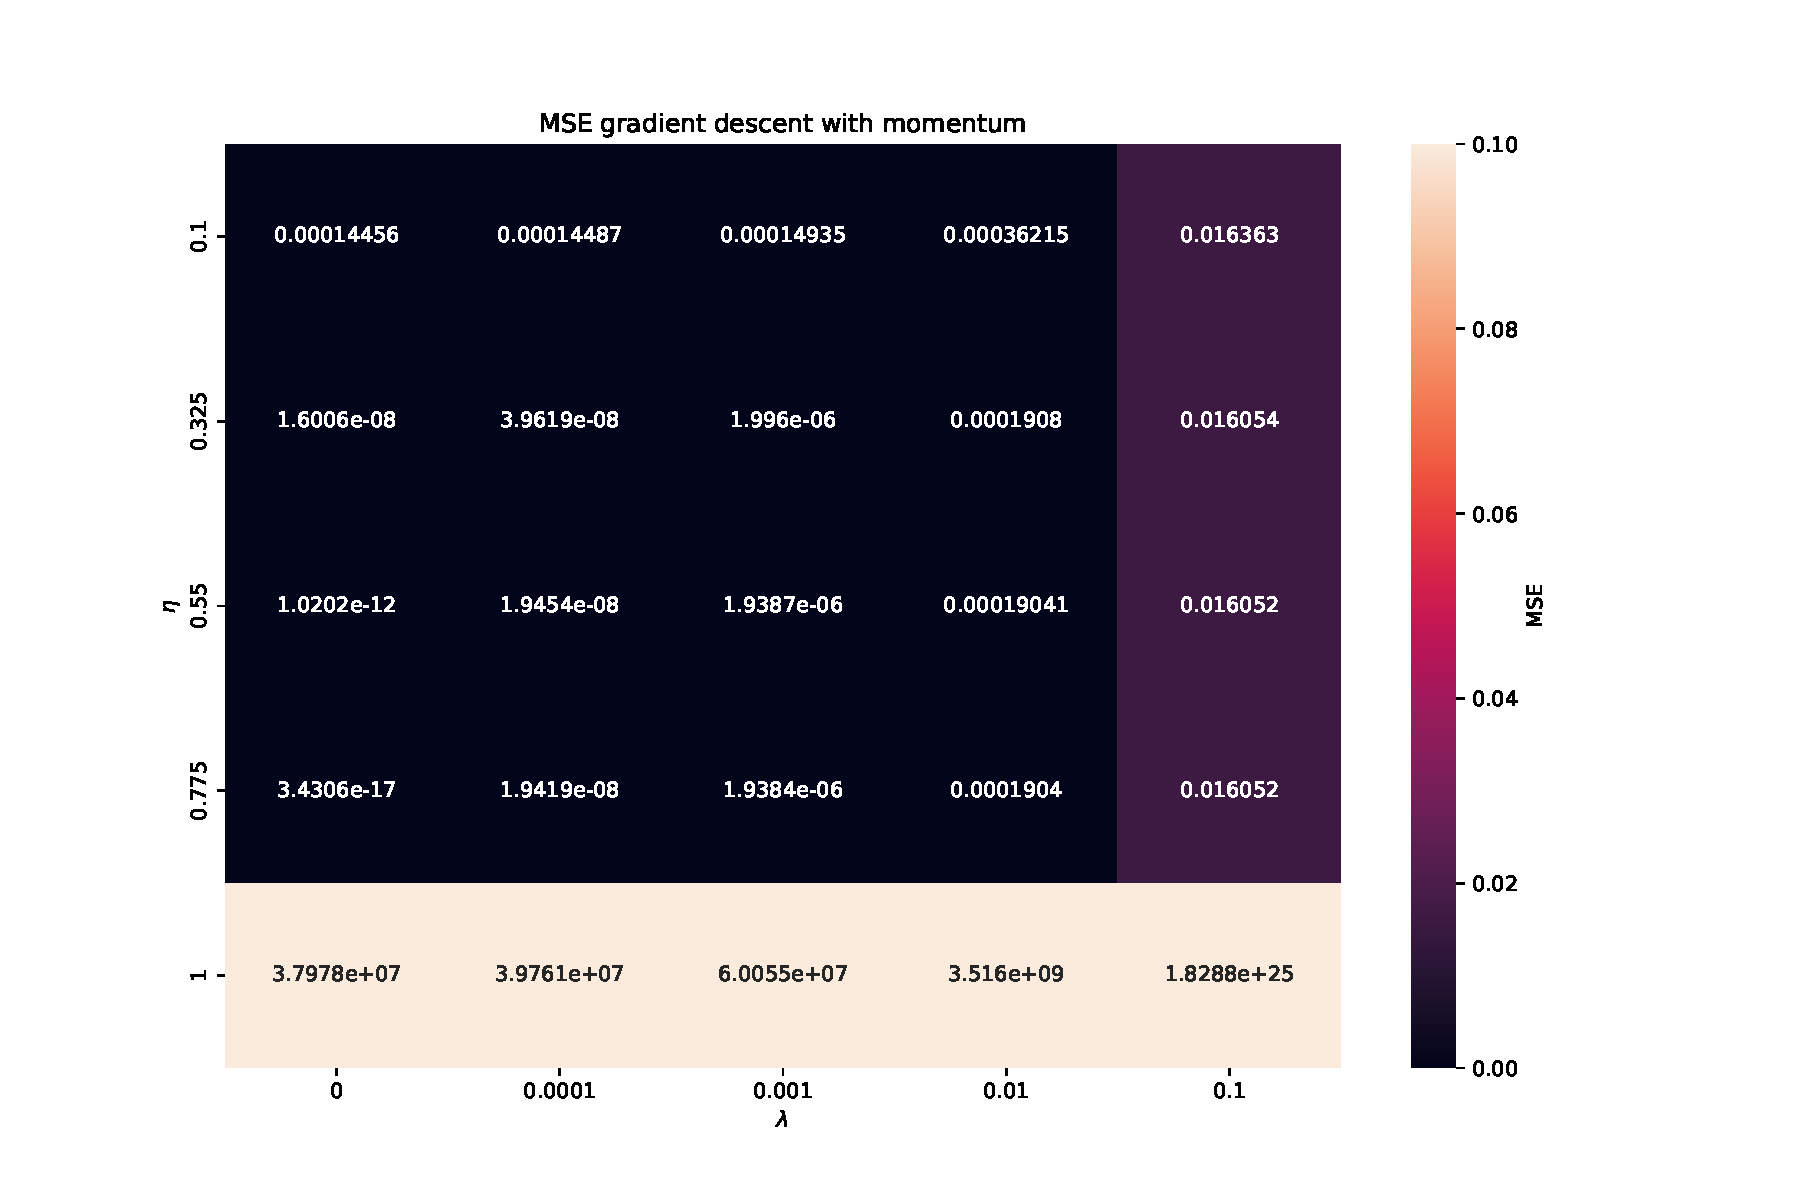
\includegraphics[width=0.8\textwidth]{Figures/PartA/gdm_MSE(eta,lmb)}
\caption{Gradient descent with momentum MSE as a function of \(\eta \) and \(\lambda \).}
\label{fig:gdm_MSE-eta-lmb-}
\end{figure}

\begin{figure}[H]
\centering
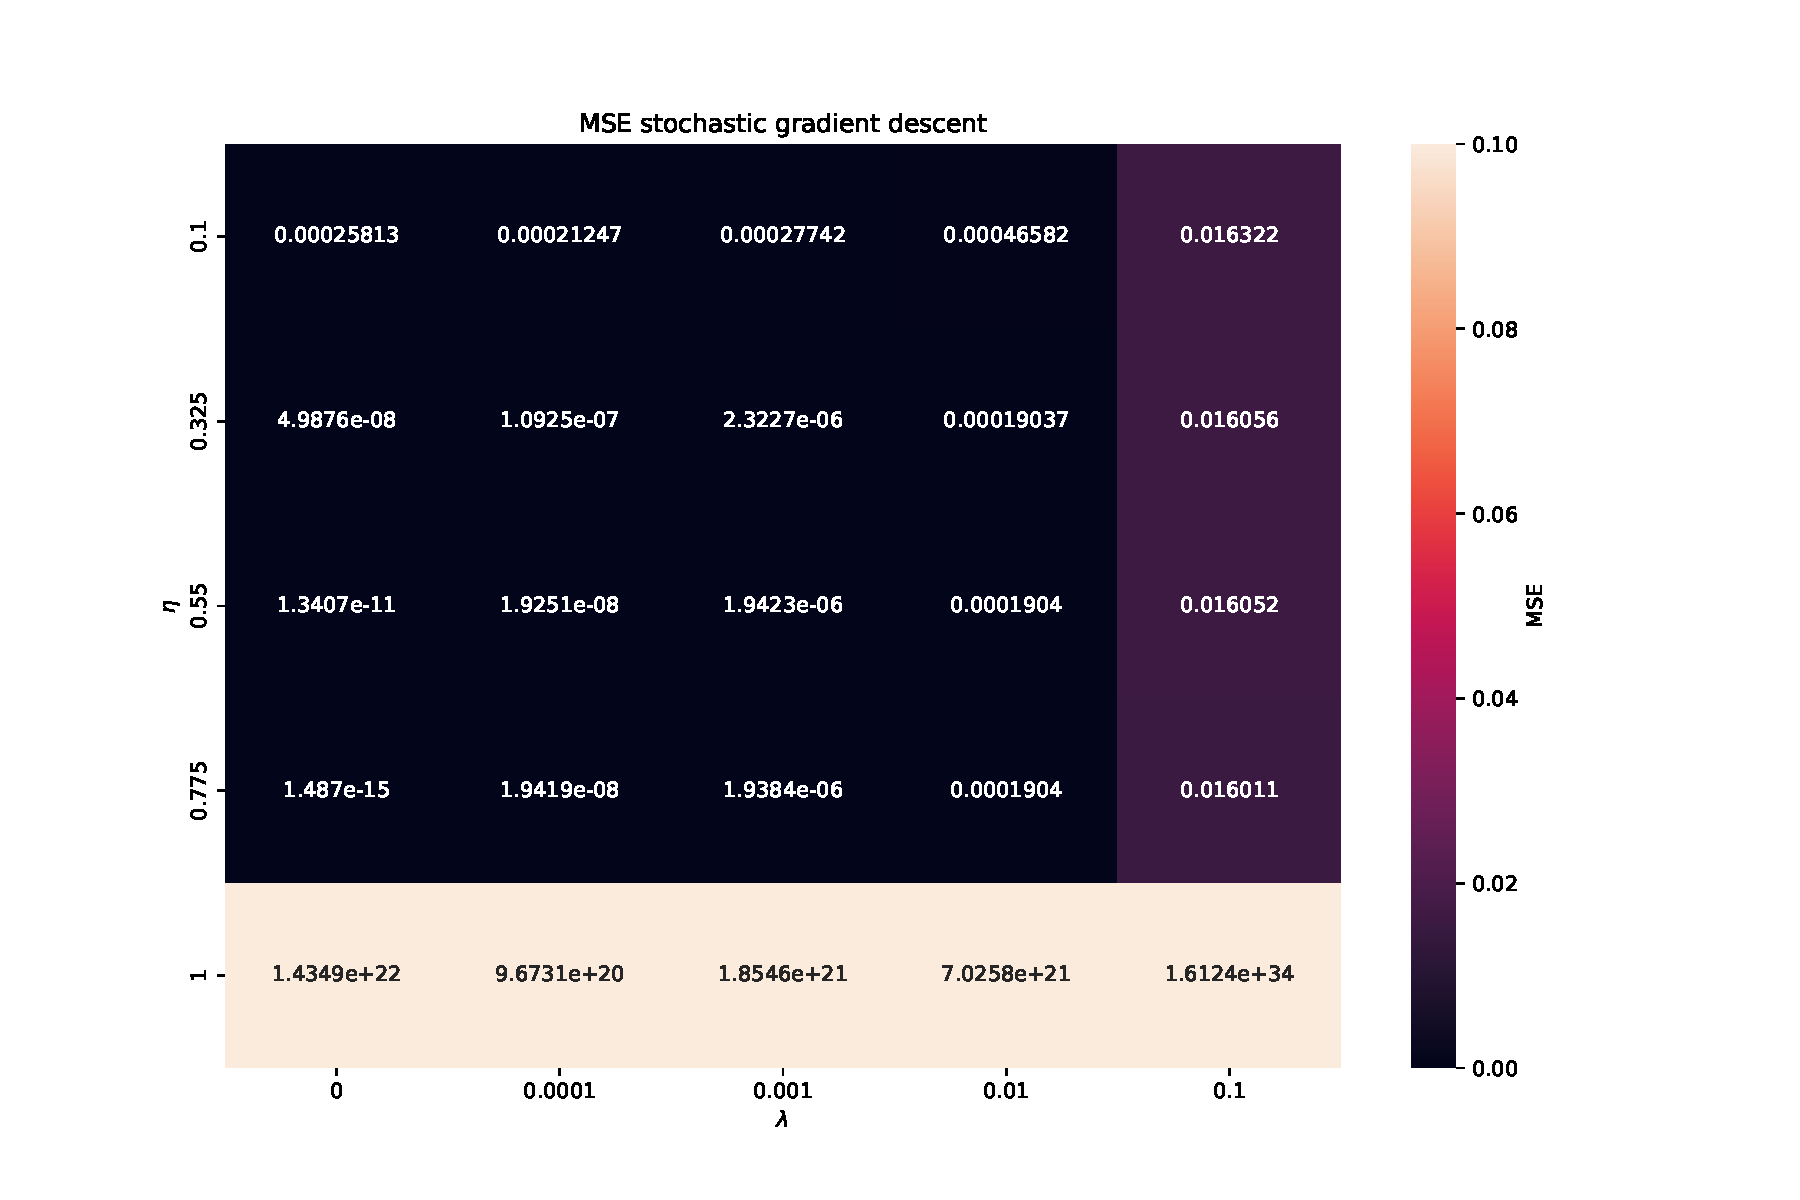
\includegraphics[width=0.8\textwidth]{Figures/PartA/sgd_MSE(eta,lmb)}
\caption{Plain stochastic gradient descent MSE as a function of \(\eta \) and \(\lambda \).}
\label{fig:sgd_MSE-eta-lmb-}
\end{figure}

\begin{figure}[H]
\centering
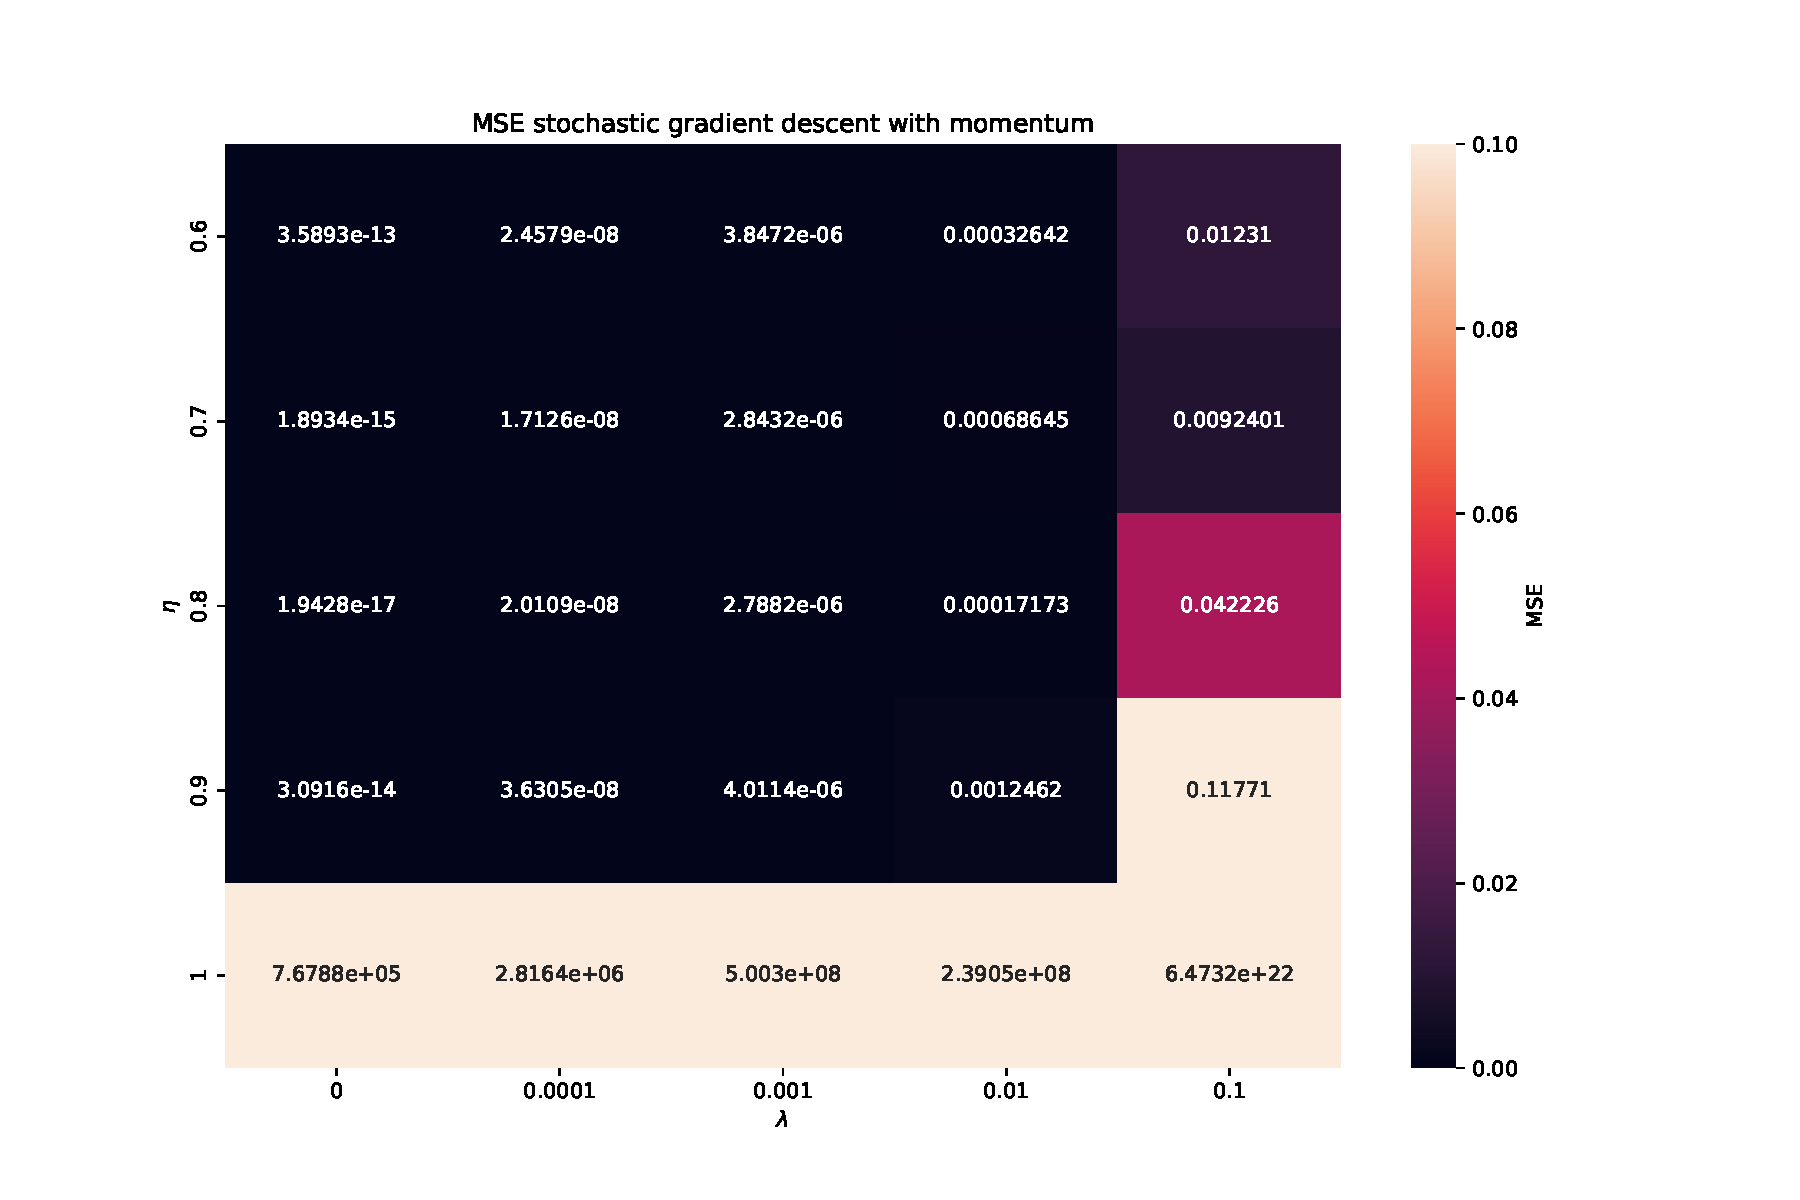
\includegraphics[width=0.8\textwidth]{Figures/PartA/sgdm_MSE(eta,lmb)}
\caption{Stochastic gradient descent with momentum MSE as a function of \(\eta \) and \(\lambda \).}
\label{fig:sgdm_MSE-eta-lmb-}
\end{figure}

Figure \ref{fig:gd_MSE-eta-lmb-}-\ref{fig:sgdm_MSE-eta-lmb-} shows MSE scores for 
stochastic gradient descent without ans with momentum, and stochastic gradient descent
without and with momentum, respectively. 
different learning rates \(\eta \) and L2-regularzation parameters \(\lambda \). 


\begin{figure}[H]
\centering
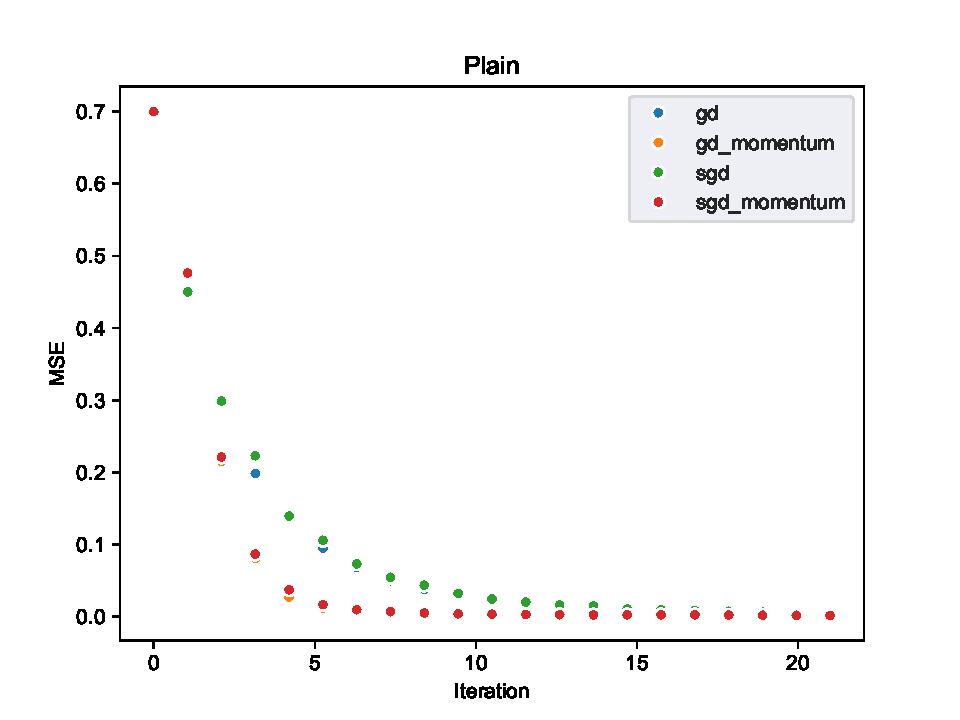
\includegraphics[width=0.8\textwidth]{Figures/PartA/PlainMSE(iter).pdf}
\caption{MSE as a function of iterations for plain and stochastic gradient descent with and without momentum}
\label{fig:PlainMSE-iter-pdf}
\end{figure}

\begin{figure}[H]
\centering
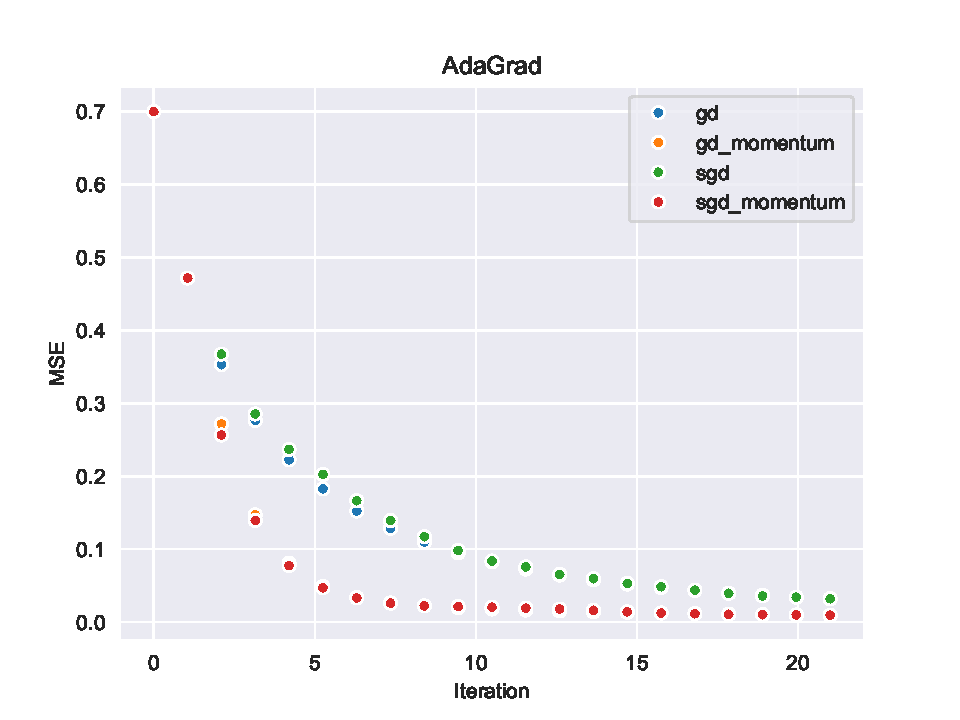
\includegraphics[width=0.8\textwidth]{Figures/PartA/AdaGradMSE(iter).pdf}
\caption{MSE as a function of iterations using tuning method AdaGrad for plain and stochastic gradient descent with and without momentum}
\label{fig:AdaGradMSE-iter-pdf}
\end{figure}

\begin{figure}[H]
\centering
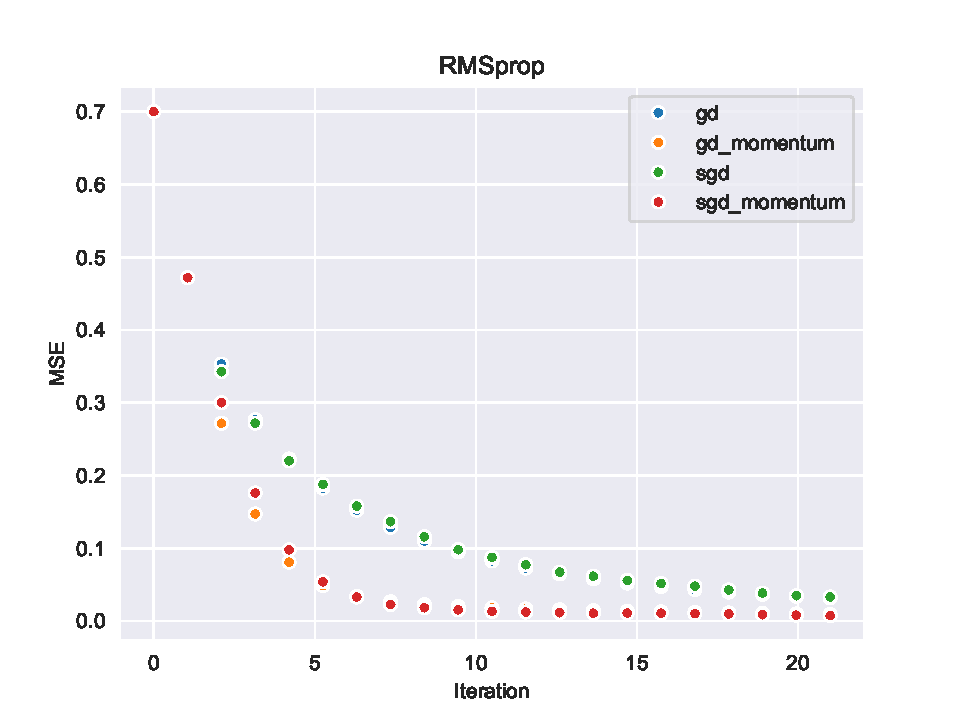
\includegraphics[width=0.8\textwidth]{Figures/PartA/RMSpropMSE(iter).pdf}
\caption{MSE as a function of iterations using tuning method RMSprop for plain and stochastic gradient descent with and without momentum}
\label{fig:RMSpropMSE-iter-pdf}
\end{figure}

\begin{figure}[H]
\centering
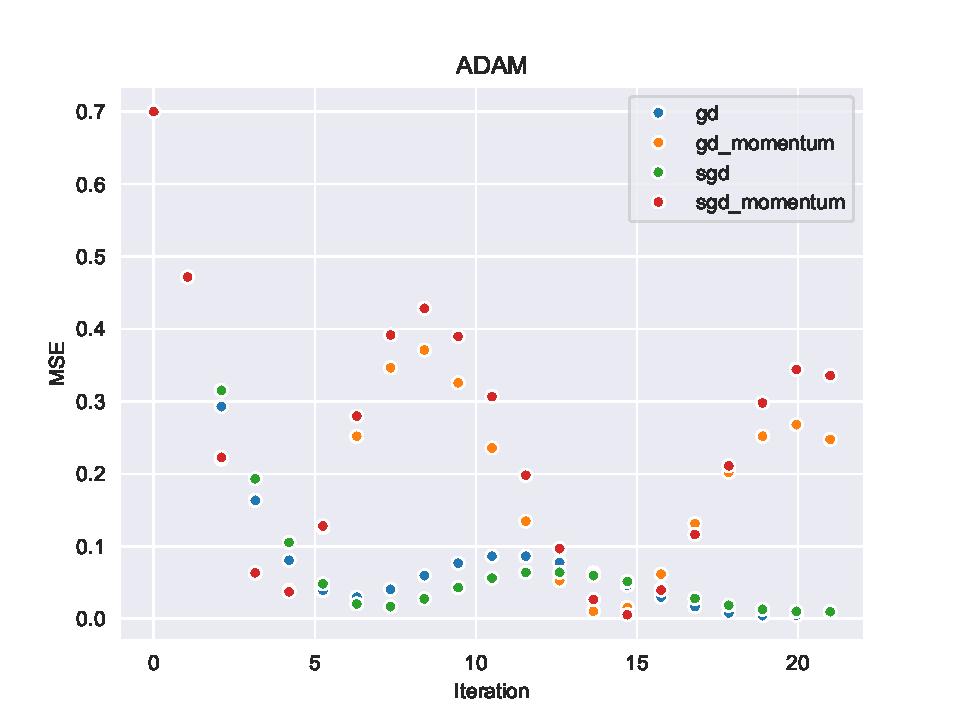
\includegraphics[width=0.8\textwidth]{Figures/PartA/ADAMMSE(iter).pdf}
\caption{MSE as a function of iterations using tuning method ADAM for plain and stochastic gradient descent with and without momentum}
\label{fig:ADAMMSE-iter-pdf}
\end{figure}



\begin{figure}[H]
\centering
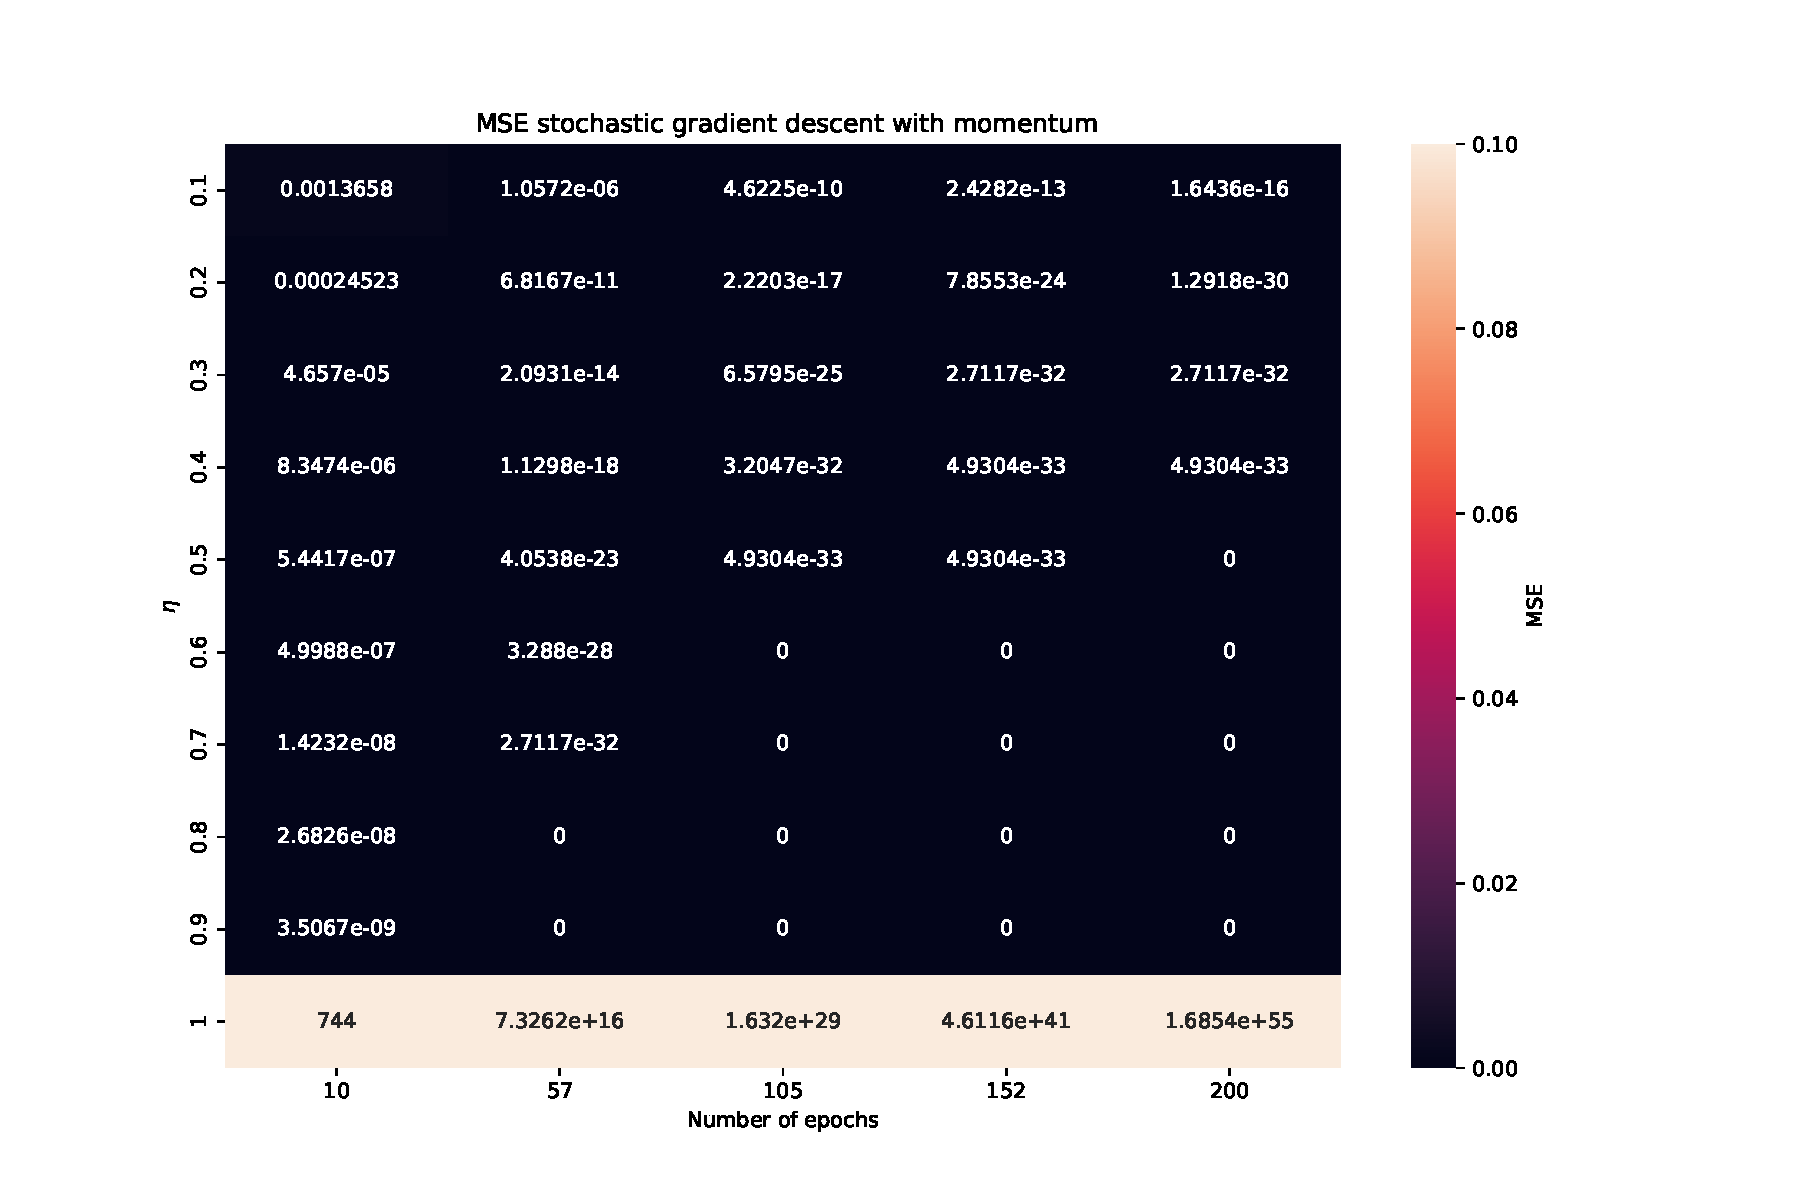
\includegraphics[width=0.8\textwidth]{Figures/PartA/_sgdm_MSE(eta,epochs)}
\caption{Stochastic gradient descent with momentum MSE as a function of epoch number and \(\eta \)	 }
\label{fig:_sgdm_MSE-eta-epochs-}
\end{figure}

\begin{figure}[H]
\centering
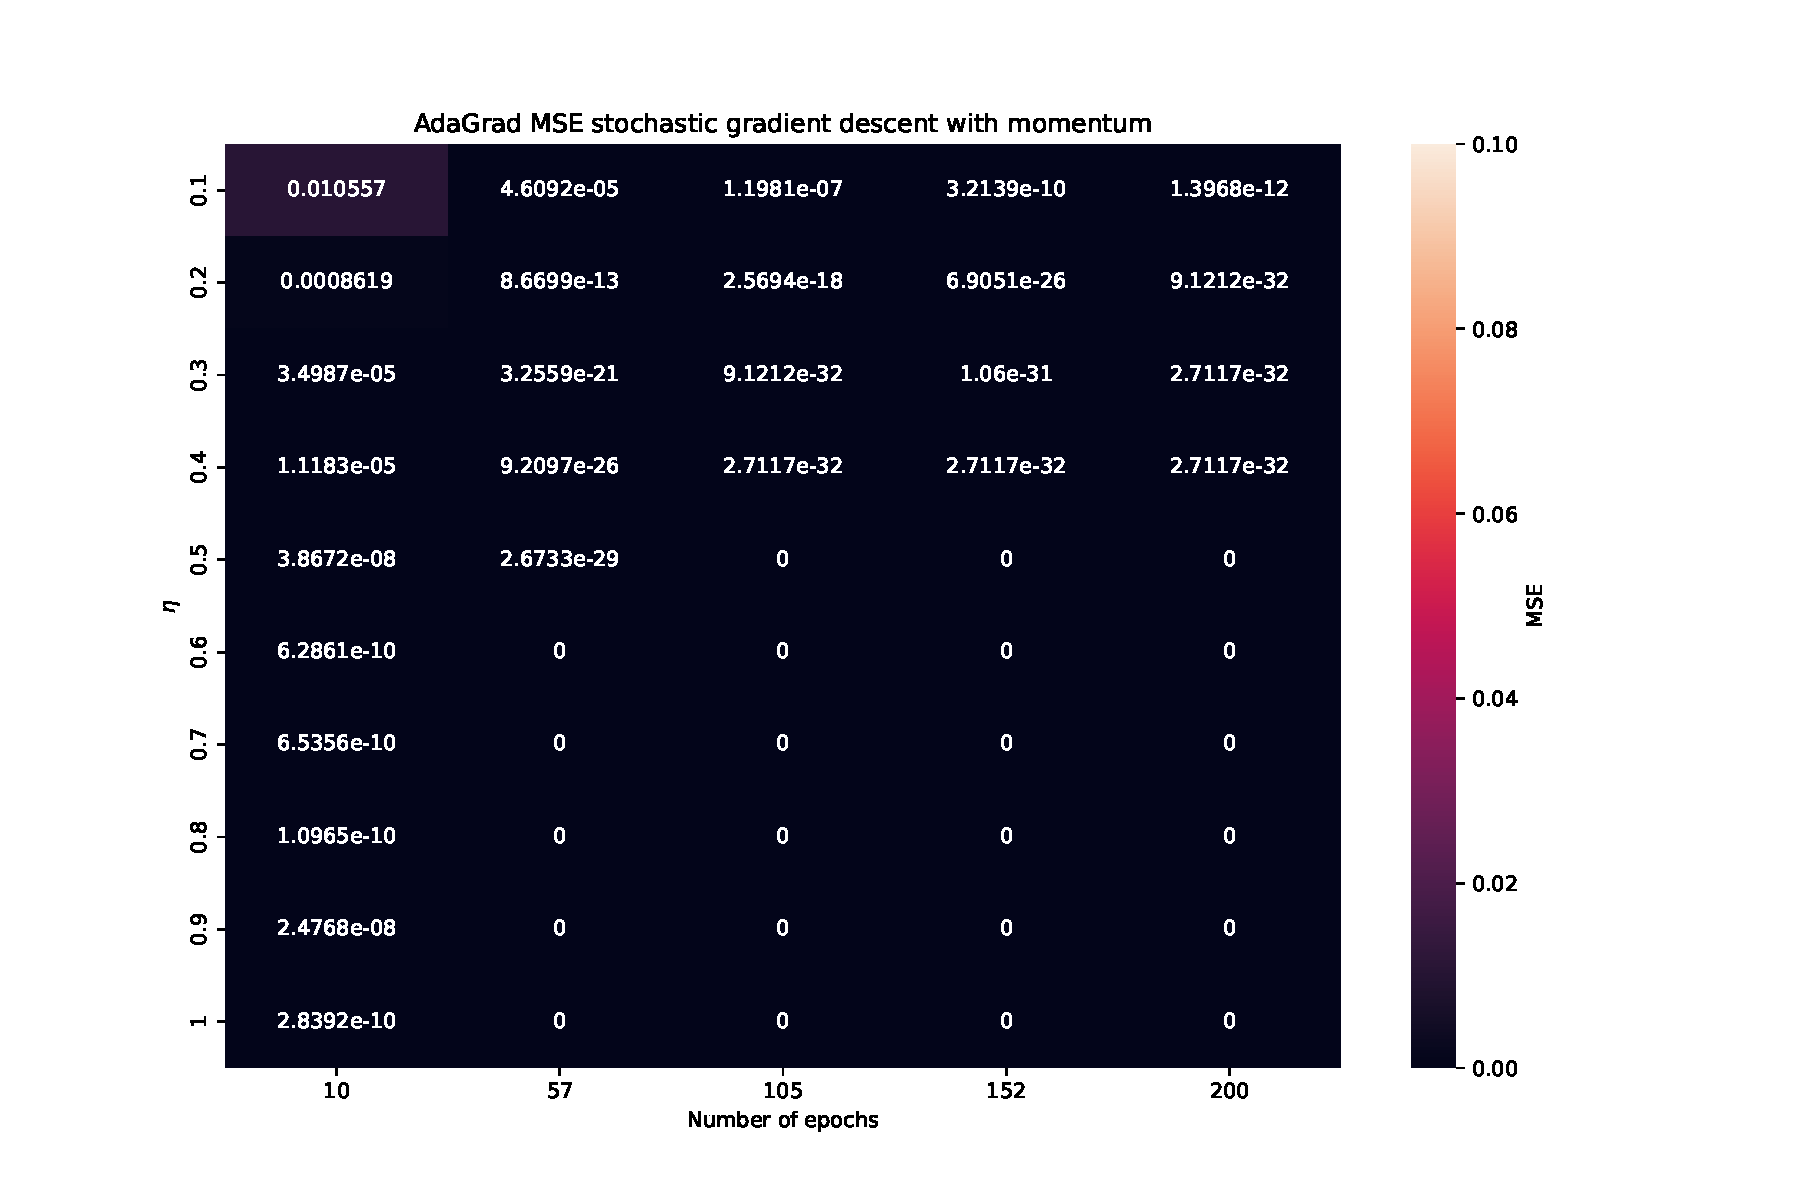
\includegraphics[width=0.8\textwidth]{Figures/PartA/AdaGrad_sgdm_MSE(eta,epochs)}
\caption{Stochastic gradient descent, with momentum and tuning method AdaGrad, MSE as a function of epoch number and \(\eta \)	 }
\label{fig:AdaGrad_sgdm_MSE-eta-epochs-}
\end{figure}

\begin{figure}[H]
\centering
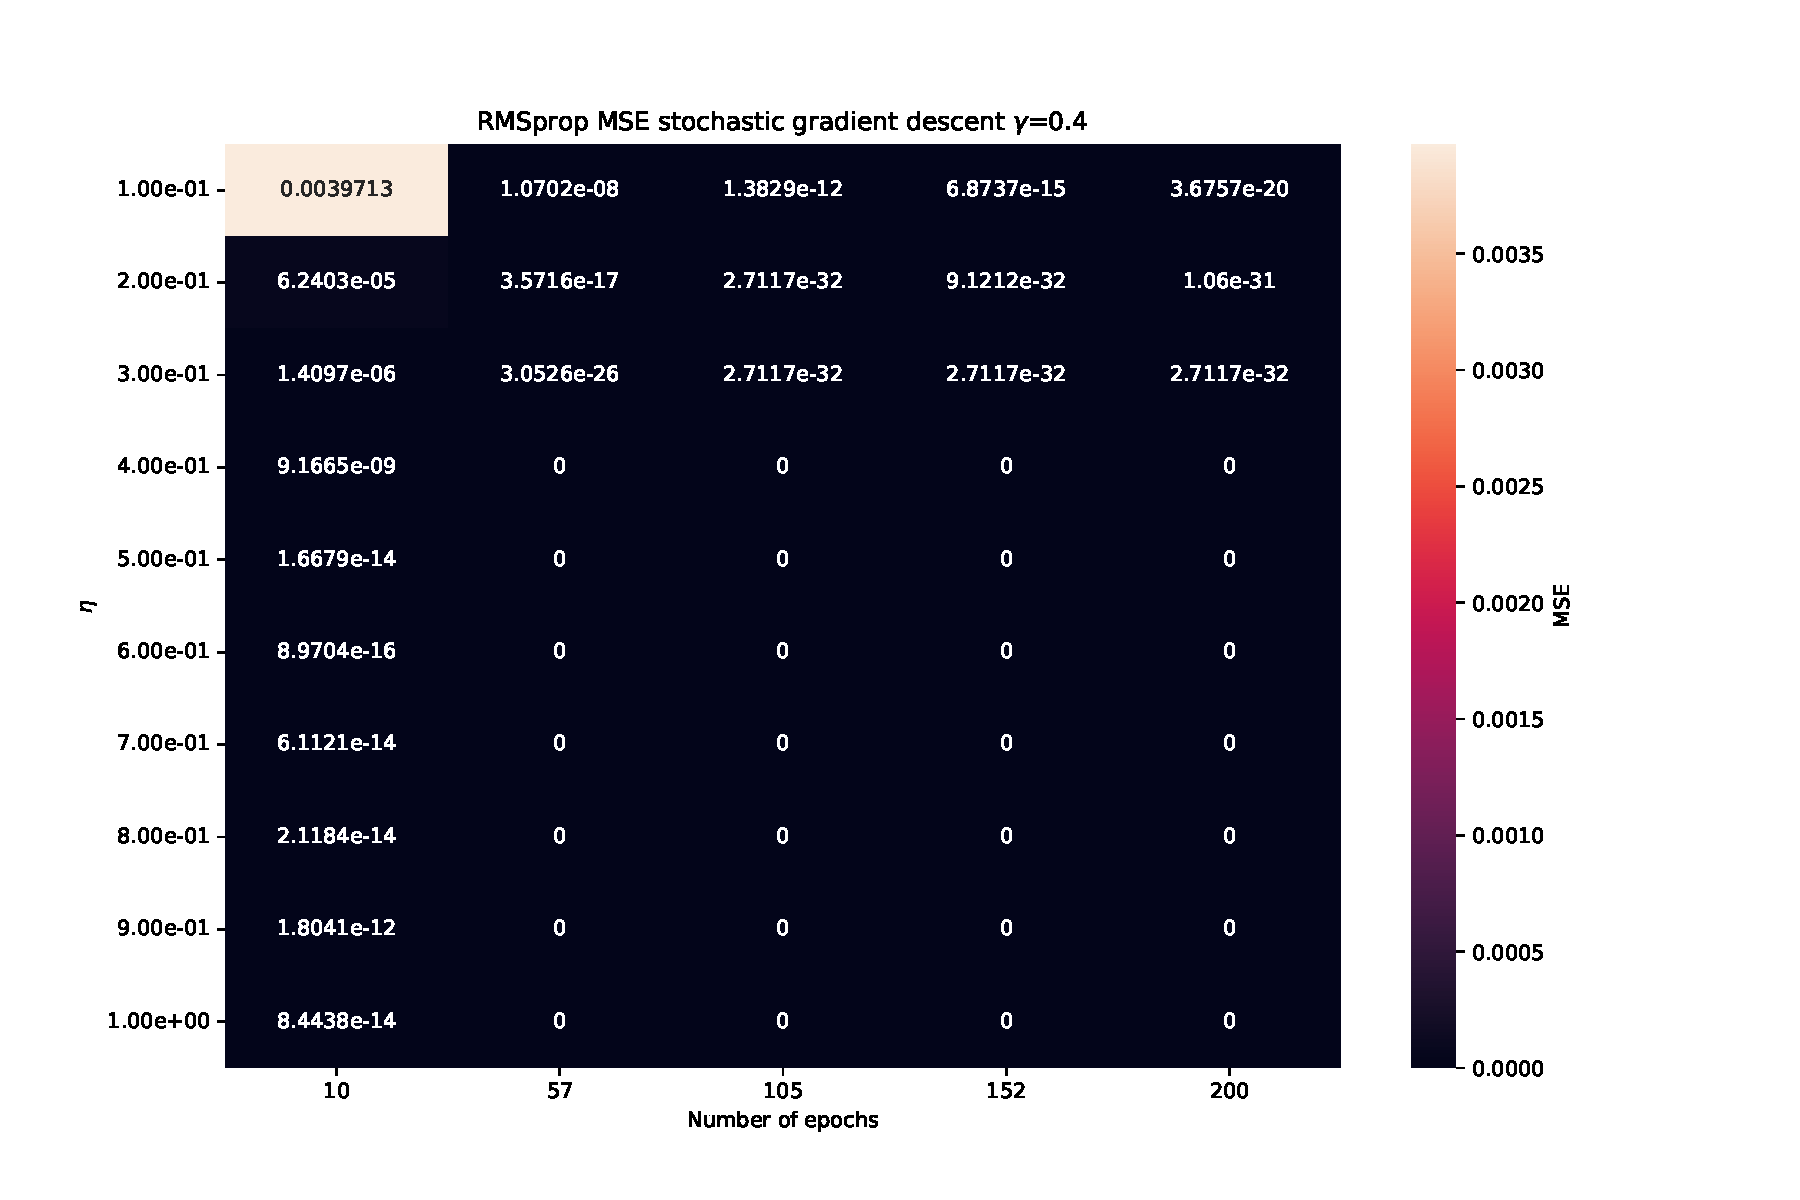
\includegraphics[width=0.8\textwidth]{Figures/PartA/RMSprop_sgdm_MSE(eta,epochs)}
\caption{Stochastic gradient descent, with momentum and tuning method RMS_prop, MSE as a function of epoch number and \(\eta \)	 }
\label{fig:RMSprop_sgdm_MSE-eta-epochs-}
\end{figure}

\begin{figure}[H]
\centering
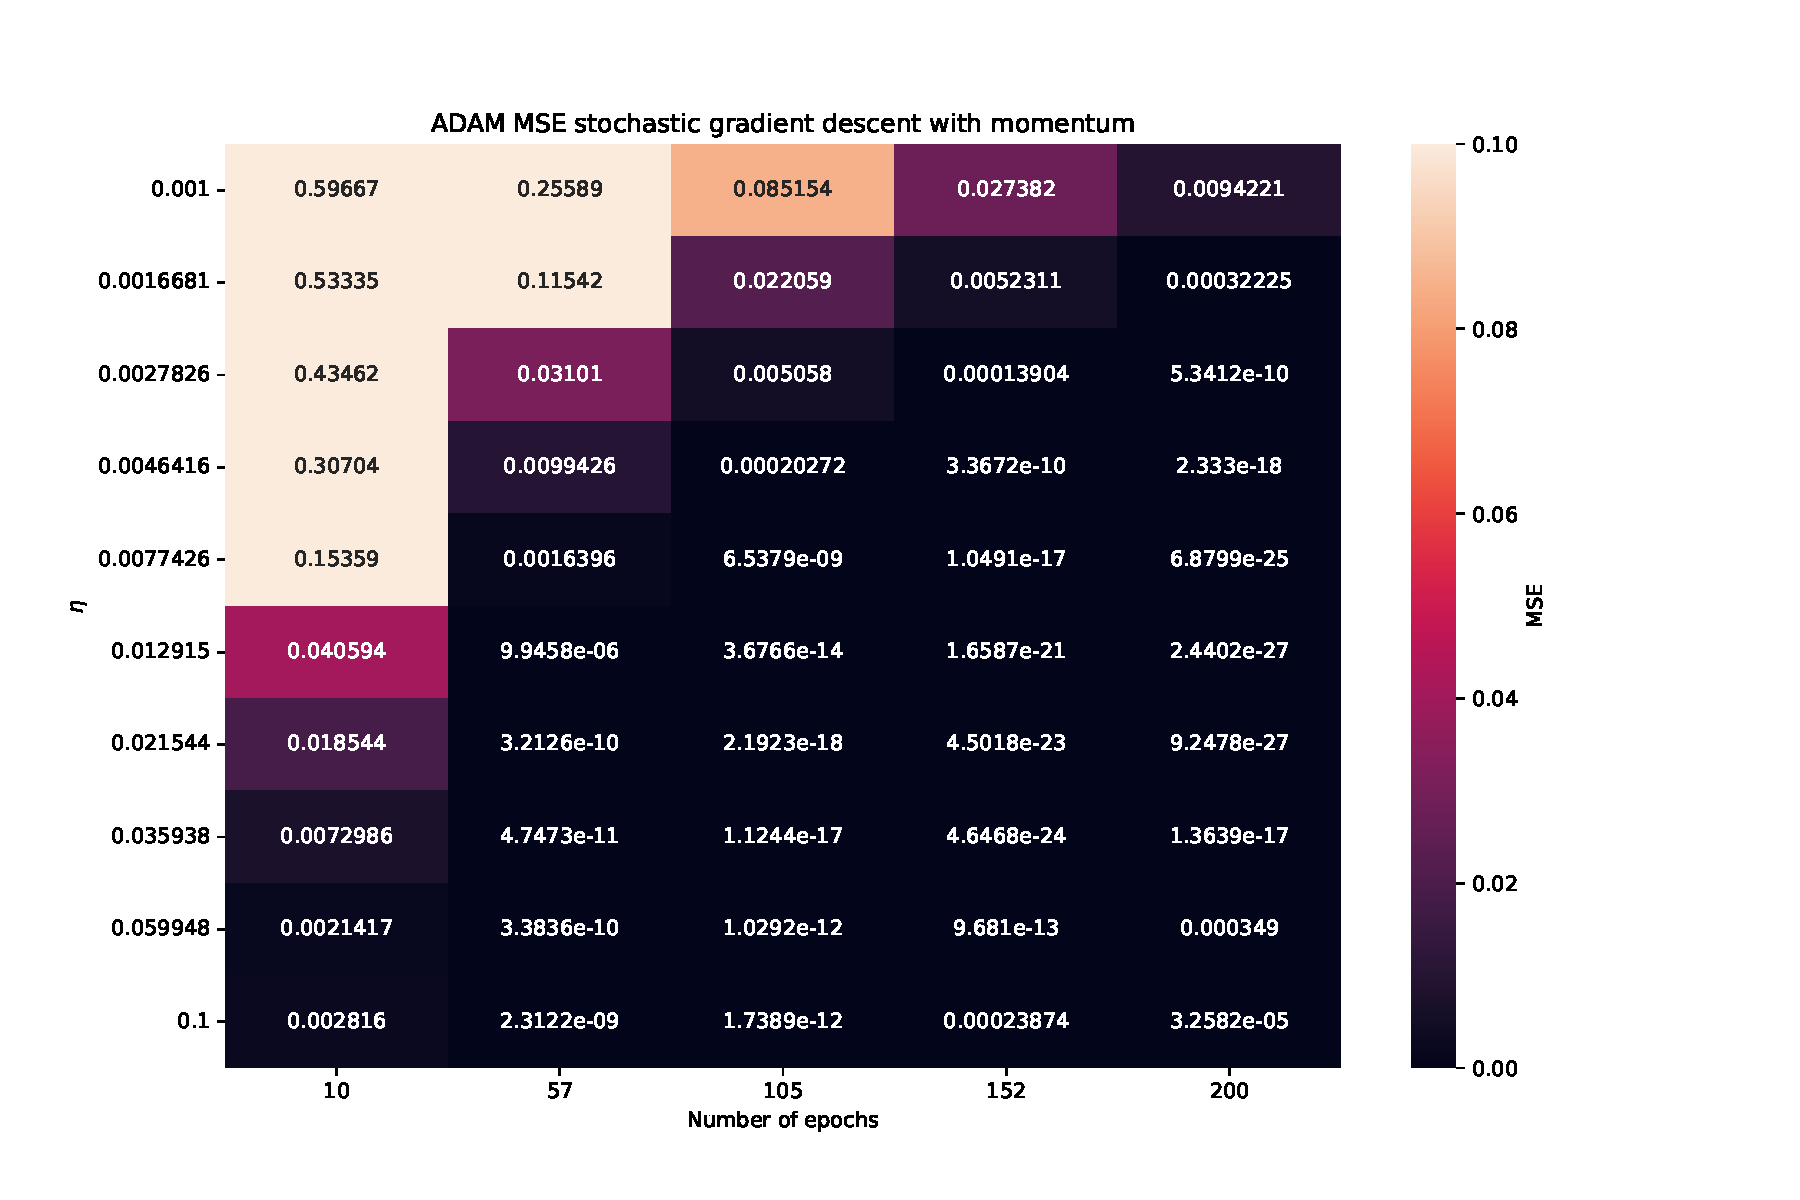
\includegraphics[width=0.8\textwidth]{Figures/PartA/ADAM_sgdm_MSE(eta,epochs)}
\caption{Stochastic gradient descent, with momentum and tuning method ADAM, MSE as a function of epoch number and \(\eta \)	 }
\label{fig:ADAM_sgdm_MSE-eta-epochs-}
\end{figure}


\subsection{Neural Network Regression}

\begin{figure}[htpb]
\begin{subfigure}{.5\textwidth}
  \centering
  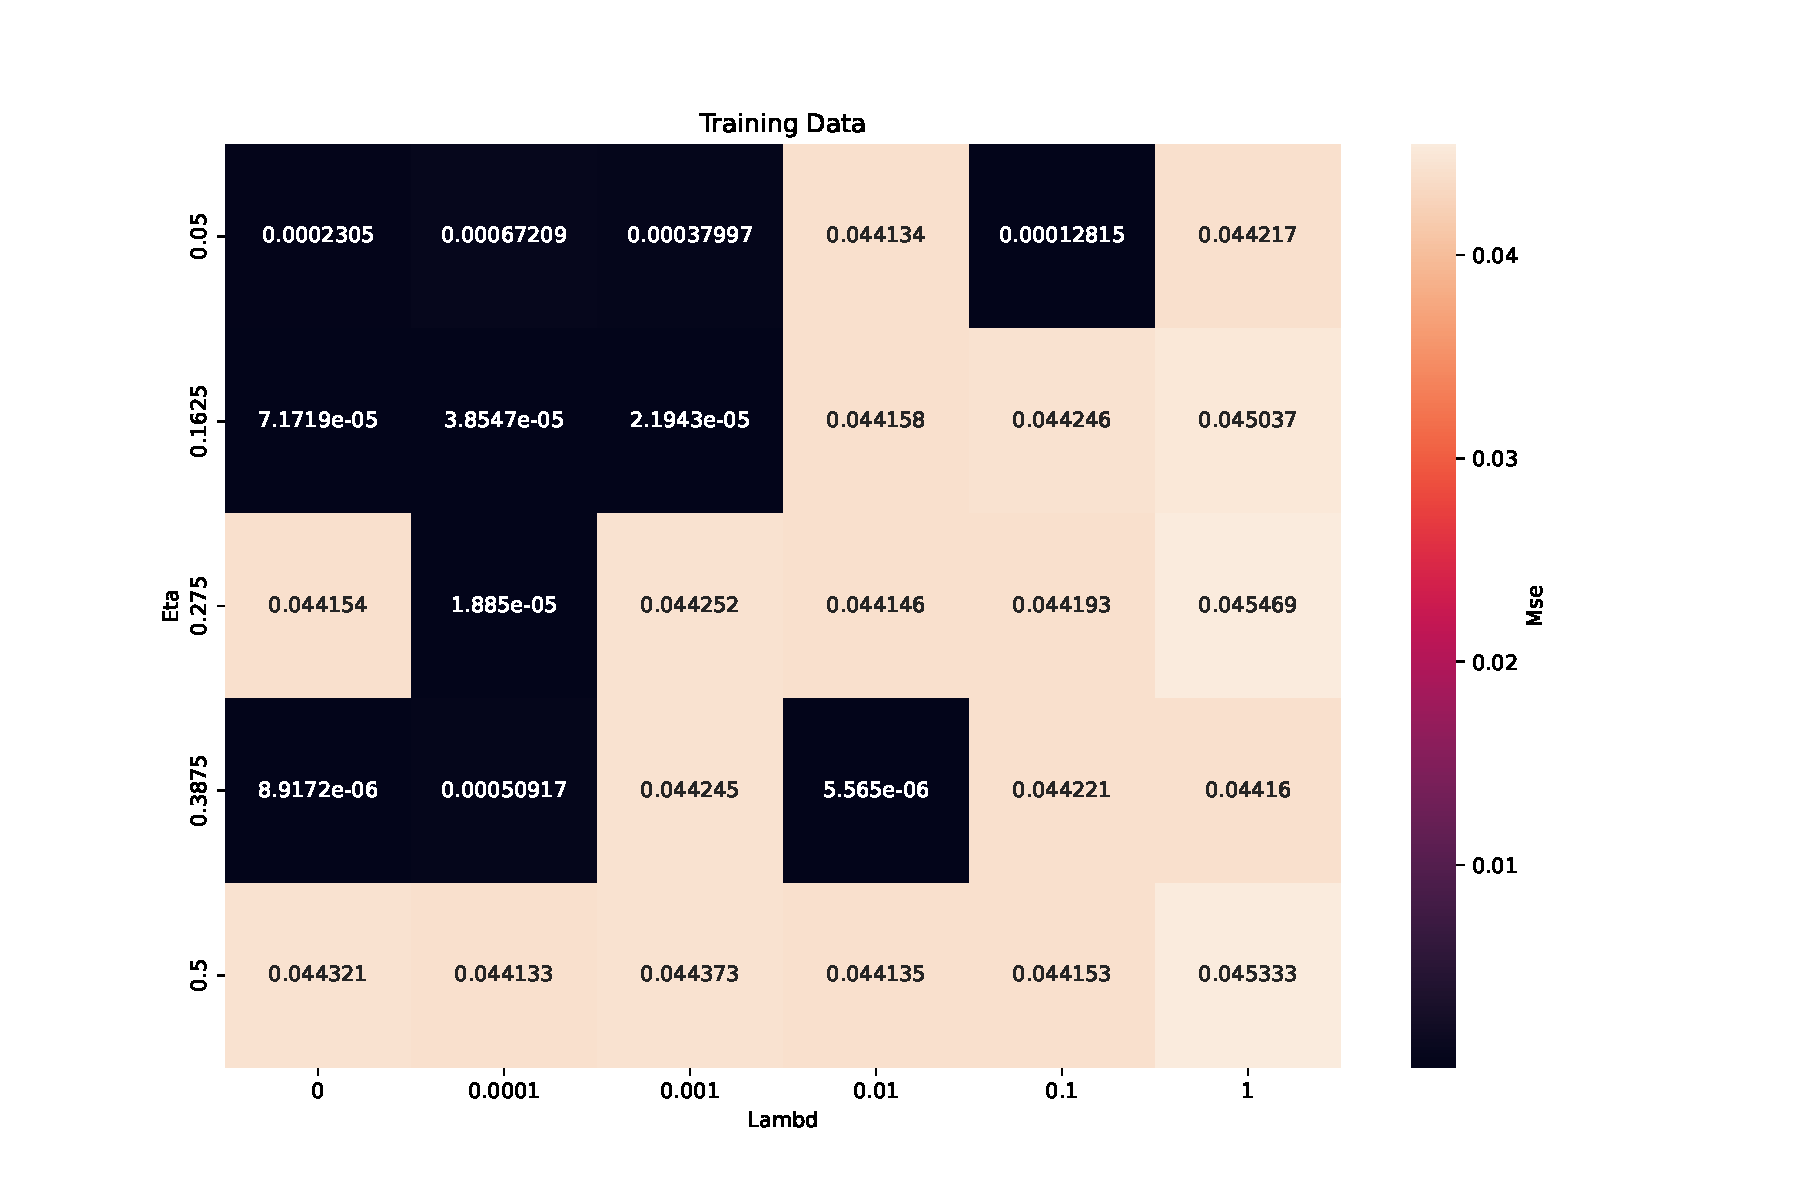
\includegraphics[width=1.2\linewidth]{Figures/PartB/train_sigmoid_MSE(eta,lmb)}
  \caption{Train MSE}
  \label{fig:train_sigmoid_MSE-eta-lmb-}
\end{subfigure}%
\begin{subfigure}{.5\textwidth}
  \centering
  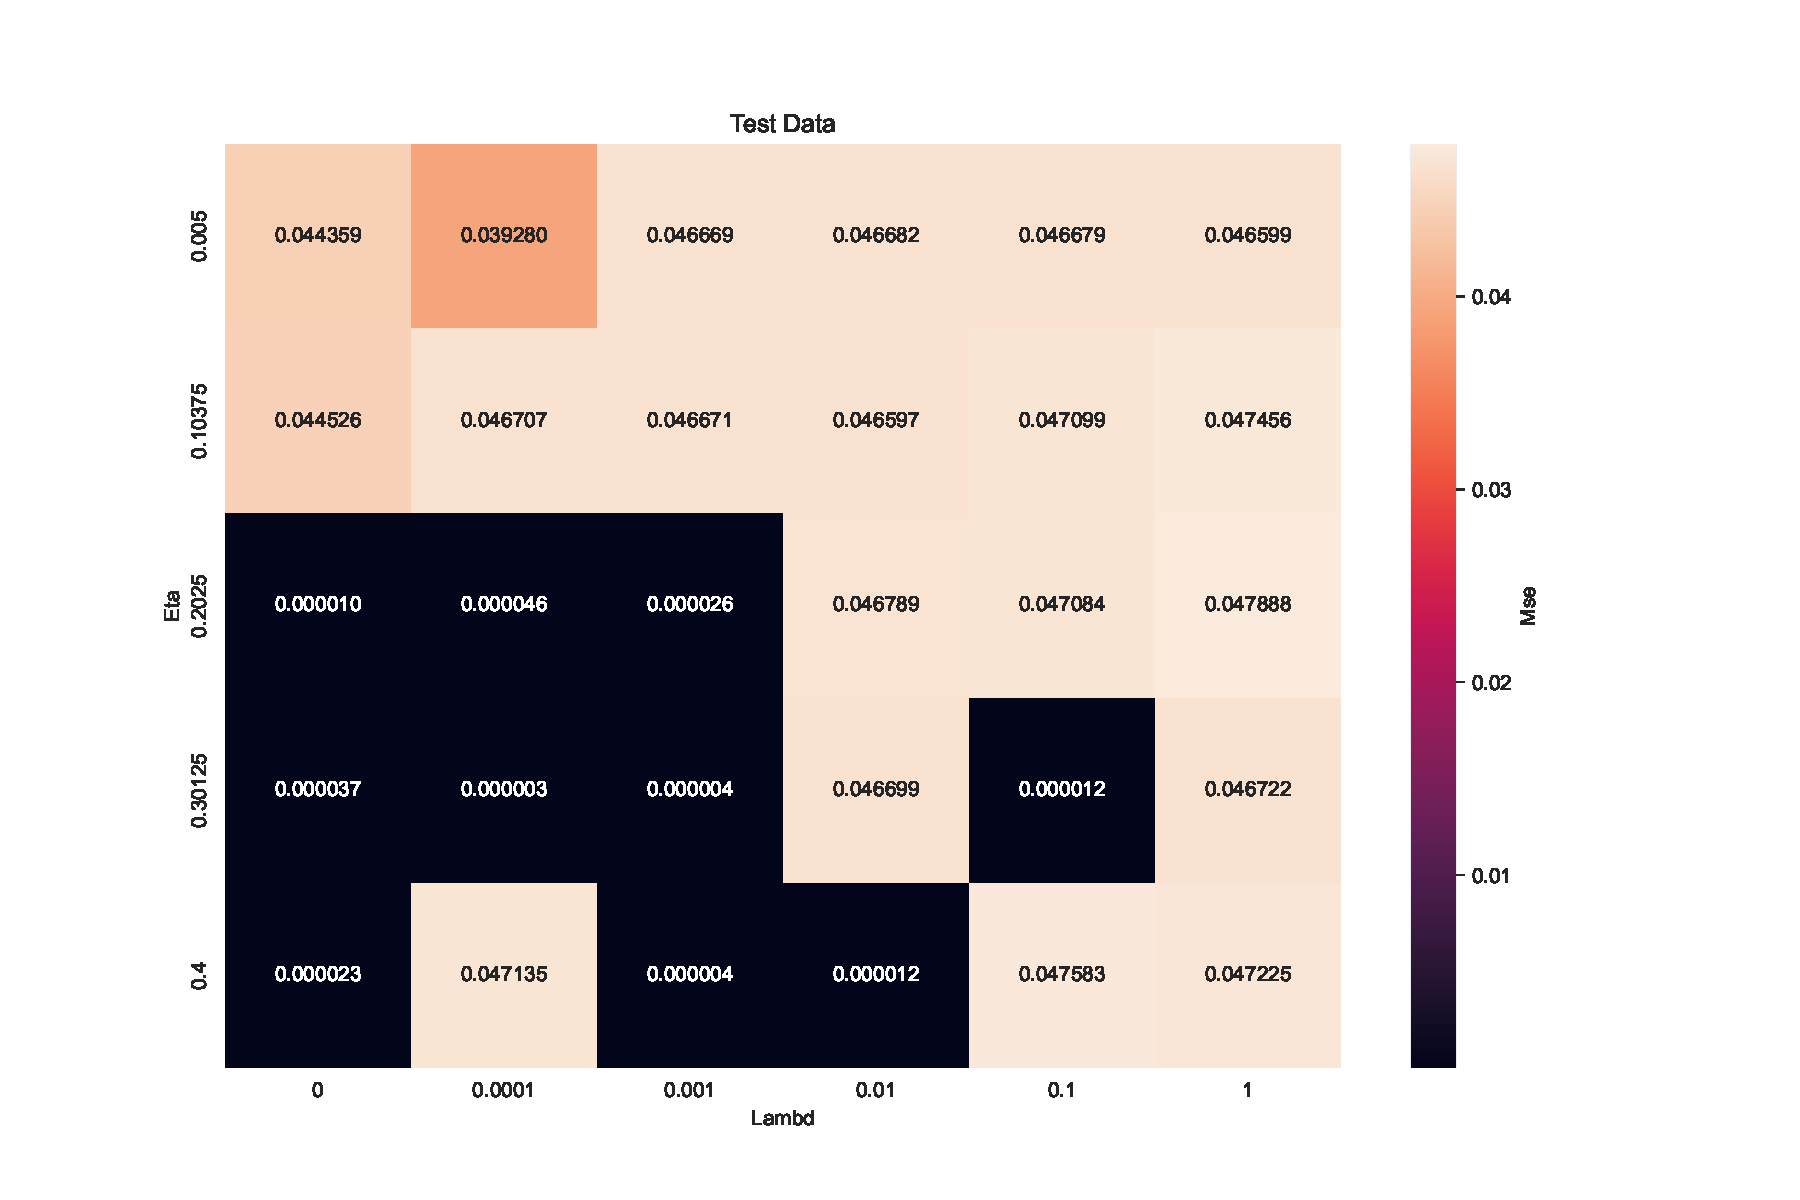
\includegraphics[width=1.2\linewidth]{Figures/PartB/test_sigmoid_MSE(eta,lmb)}
  \caption{Test MSE}
  \label{fig:test_sigmoid_MSE-eta-lmb-}
\end{subfigure}
\caption{Neural network with activation function Sigmoid MSE as a function of \(\eta \) and \(\lambda \) }
\label{fig:Sigmoid_MSE}
\end{figure}

\begin{figure}[htpb]
\begin{subfigure}{.5\textwidth}
  \centering
  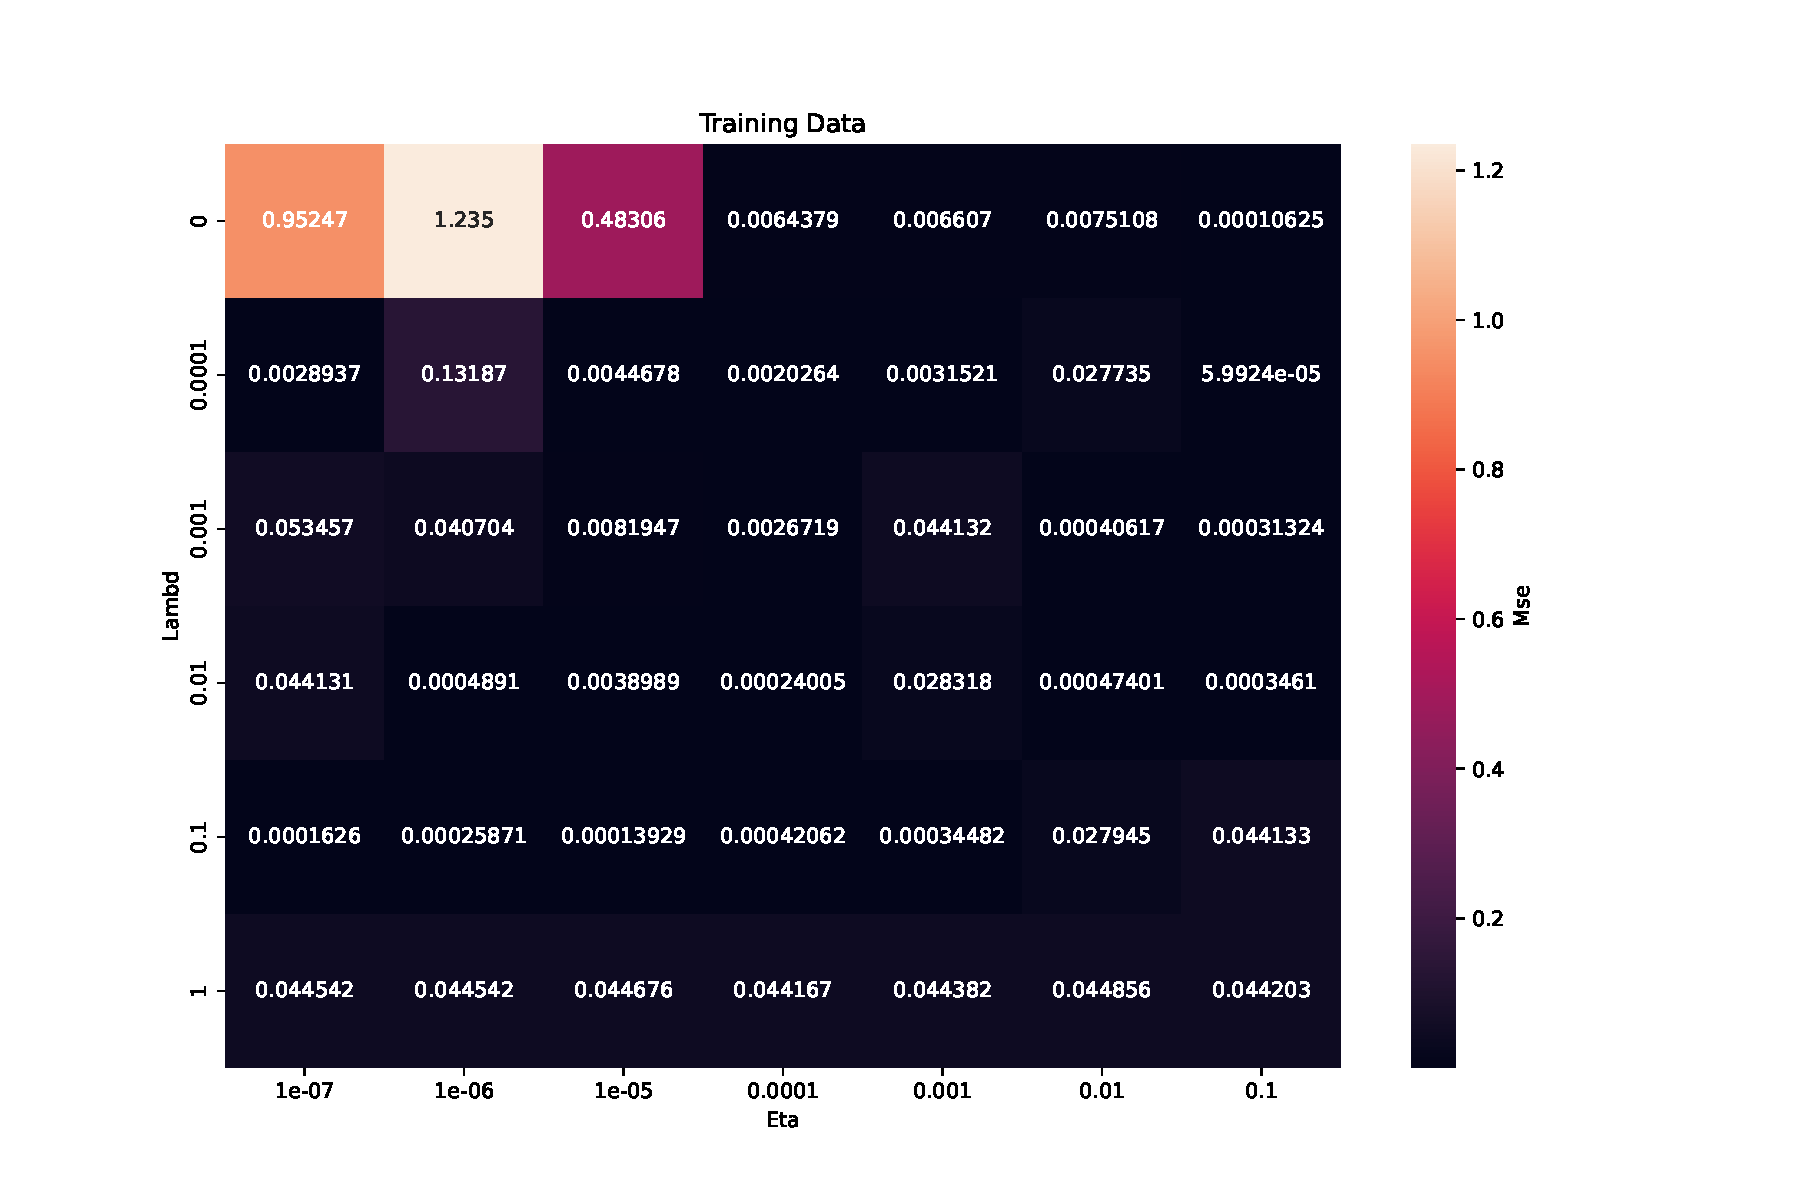
\includegraphics[width=1.2\linewidth]{Figures/PartB/train_relu_MSE(eta,lmb)}
  \caption{Train MSE}
  \label{fig:train_relu_MSE-eta-lmb-}
\end{subfigure}%
\begin{subfigure}{.5\textwidth}
  \centering
  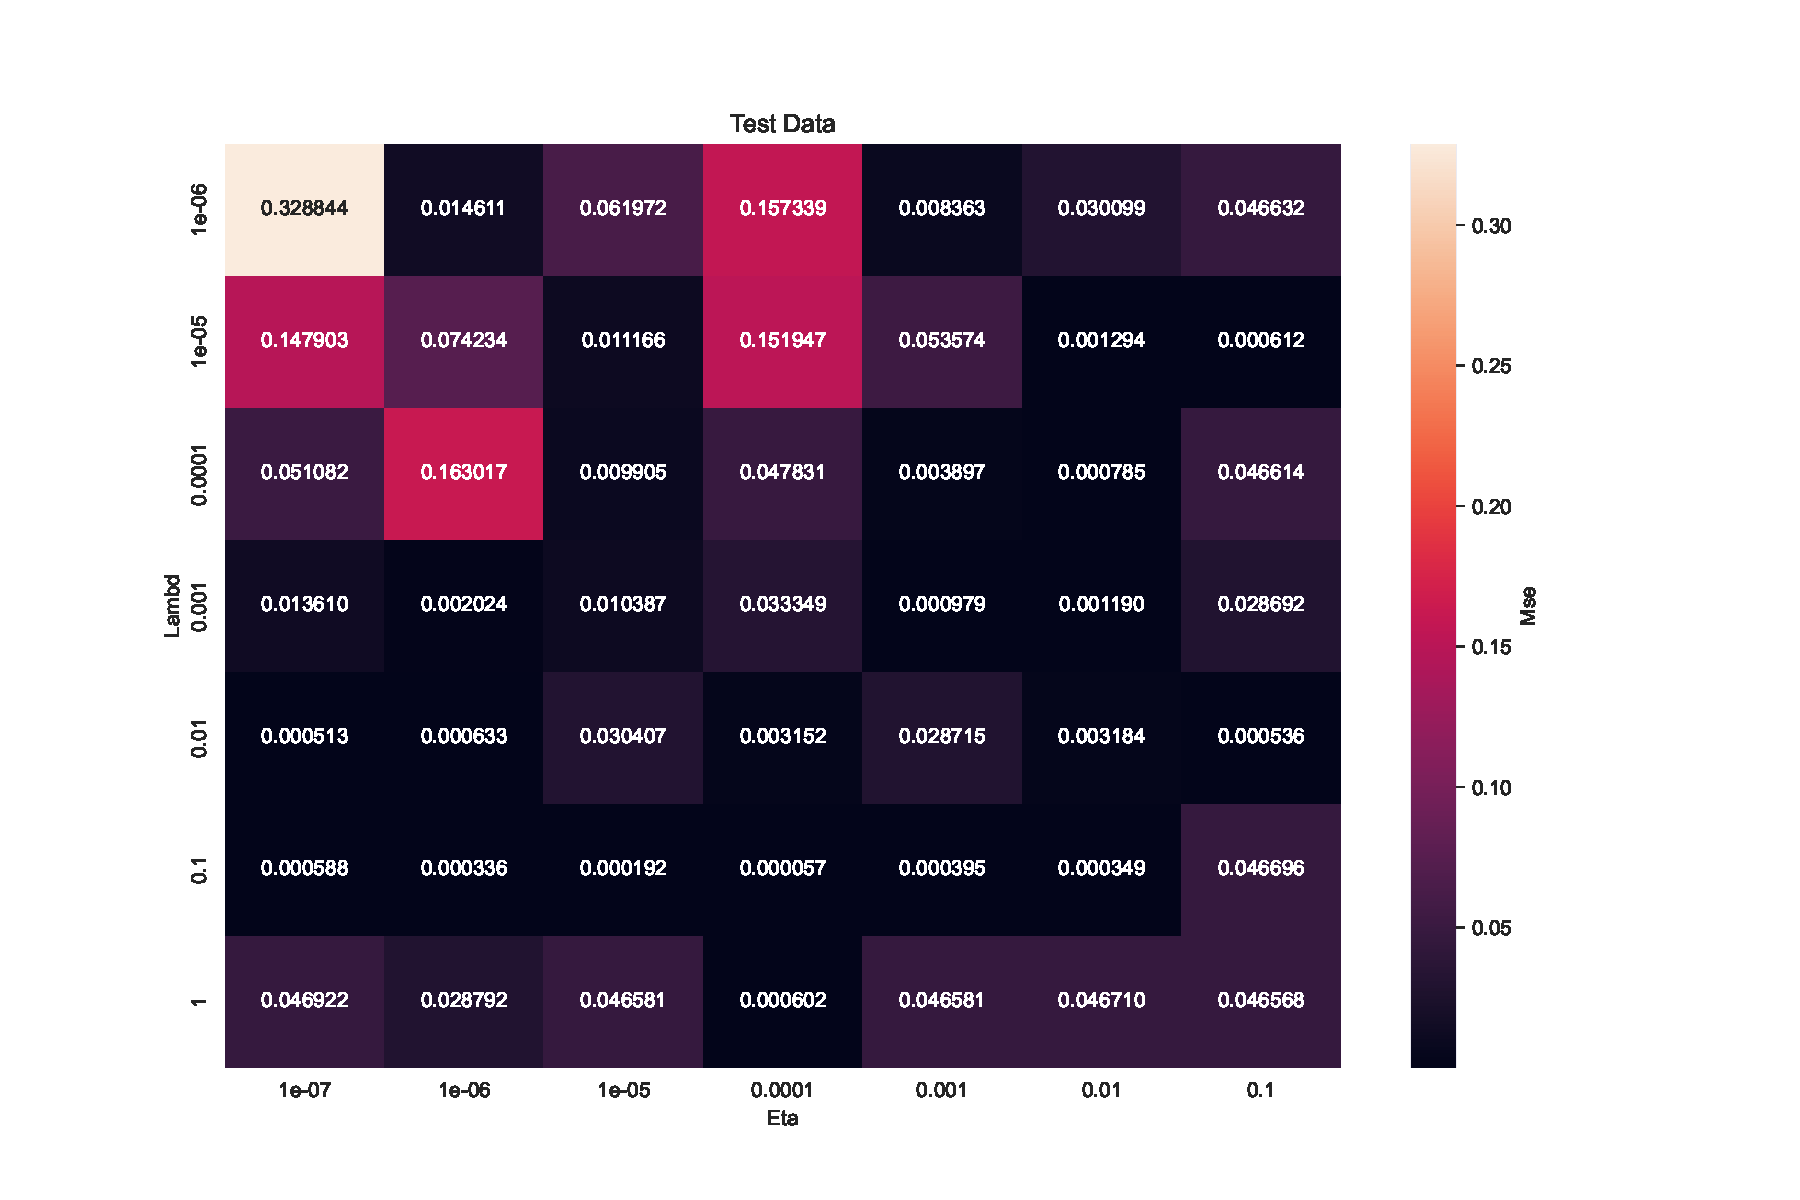
\includegraphics[width=1.2\linewidth]{Figures/PartB/test_relu_MSE(eta,lmb)}
  \caption{Test MSE}
  \label{fig:test_relu_MSE-eta-lmb-}
\end{subfigure}
\caption{Neural network with activation function relu MSE as a function of \(\eta \) and \(\lambda \) }
\label{fig:relu_MSE}
\end{figure}

\begin{figure}[htpb]
\begin{subfigure}{.5\textwidth}
  \centering
  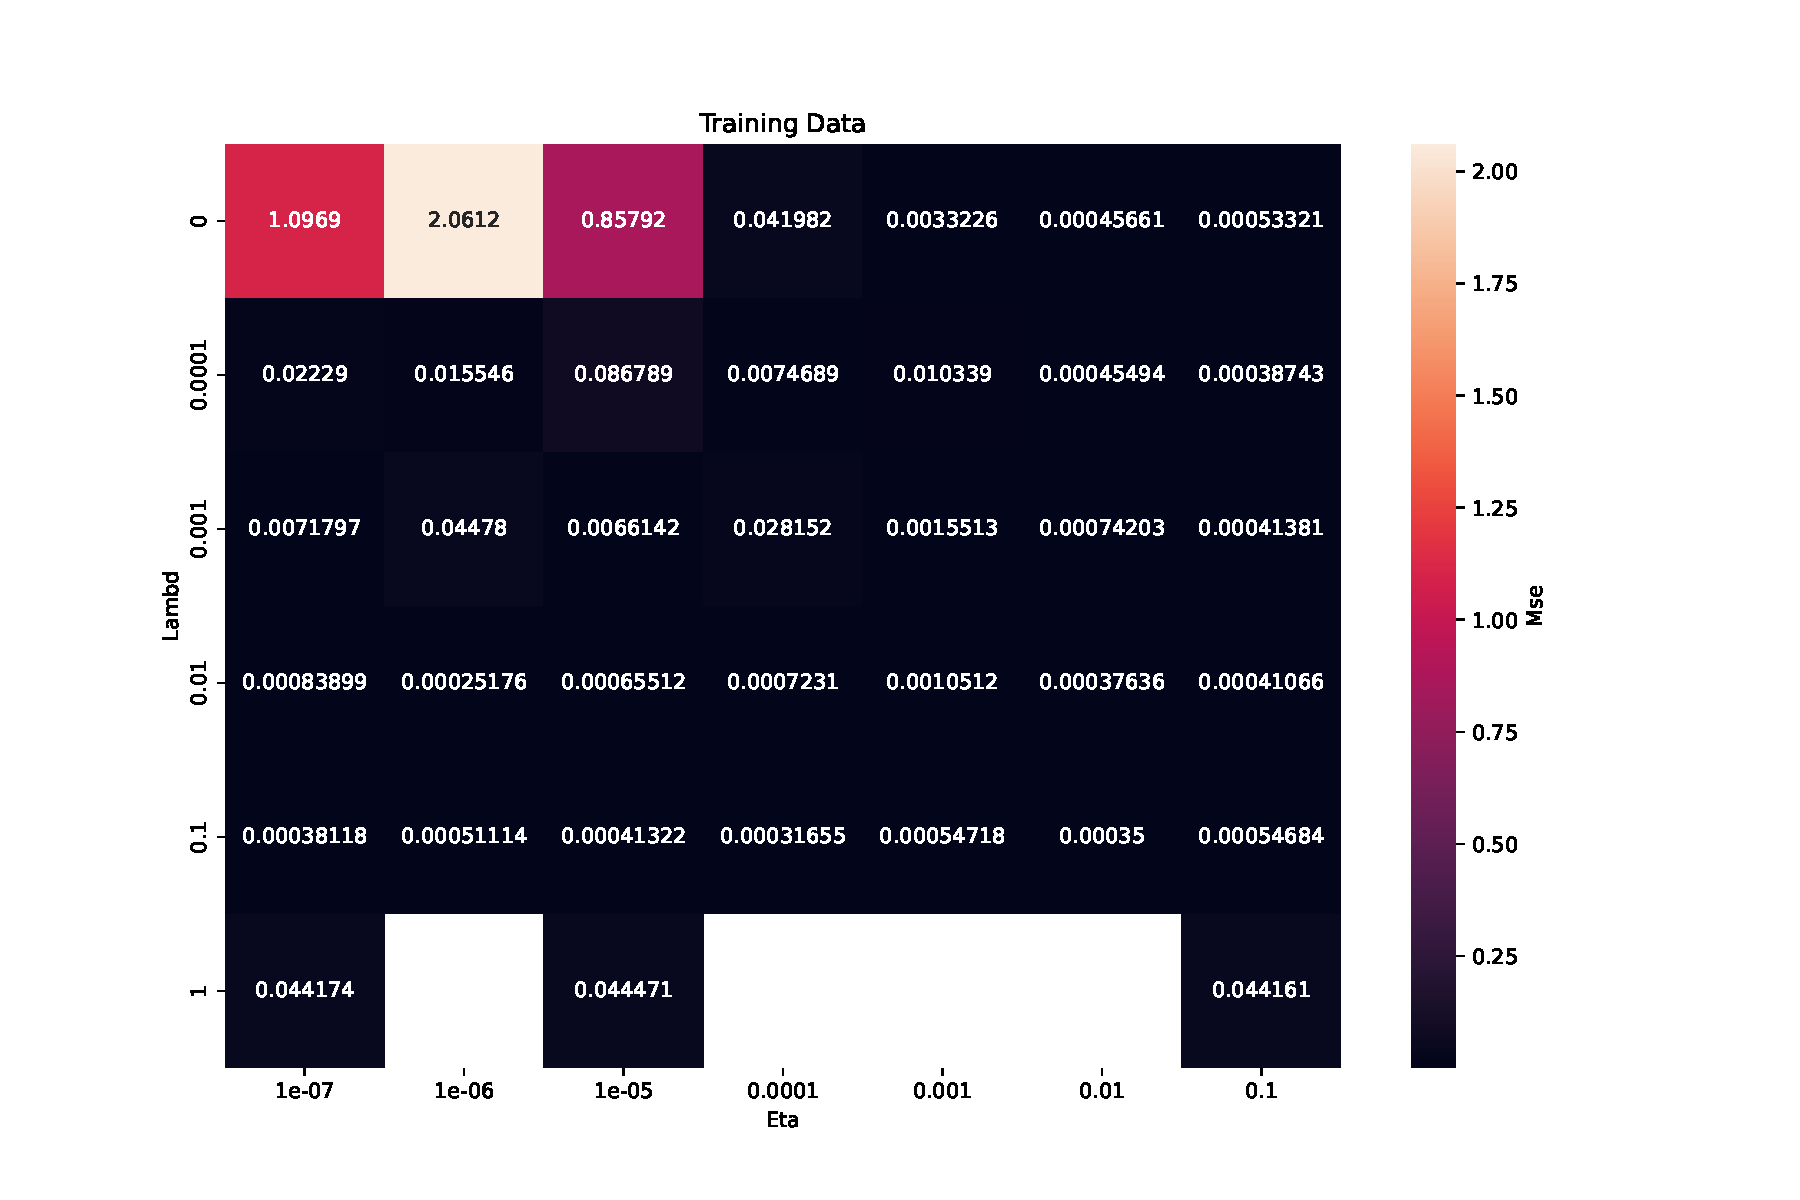
\includegraphics[width=1.2\linewidth]{Figures/PartB/train_leaky_relu_MSE(eta,lmb)}
  \caption{Train MSE}
  \label{fig:train_leaky_relu_MSE-eta-lmb-}
\end{subfigure}%
\begin{subfigure}{.5\textwidth}
  \centering
  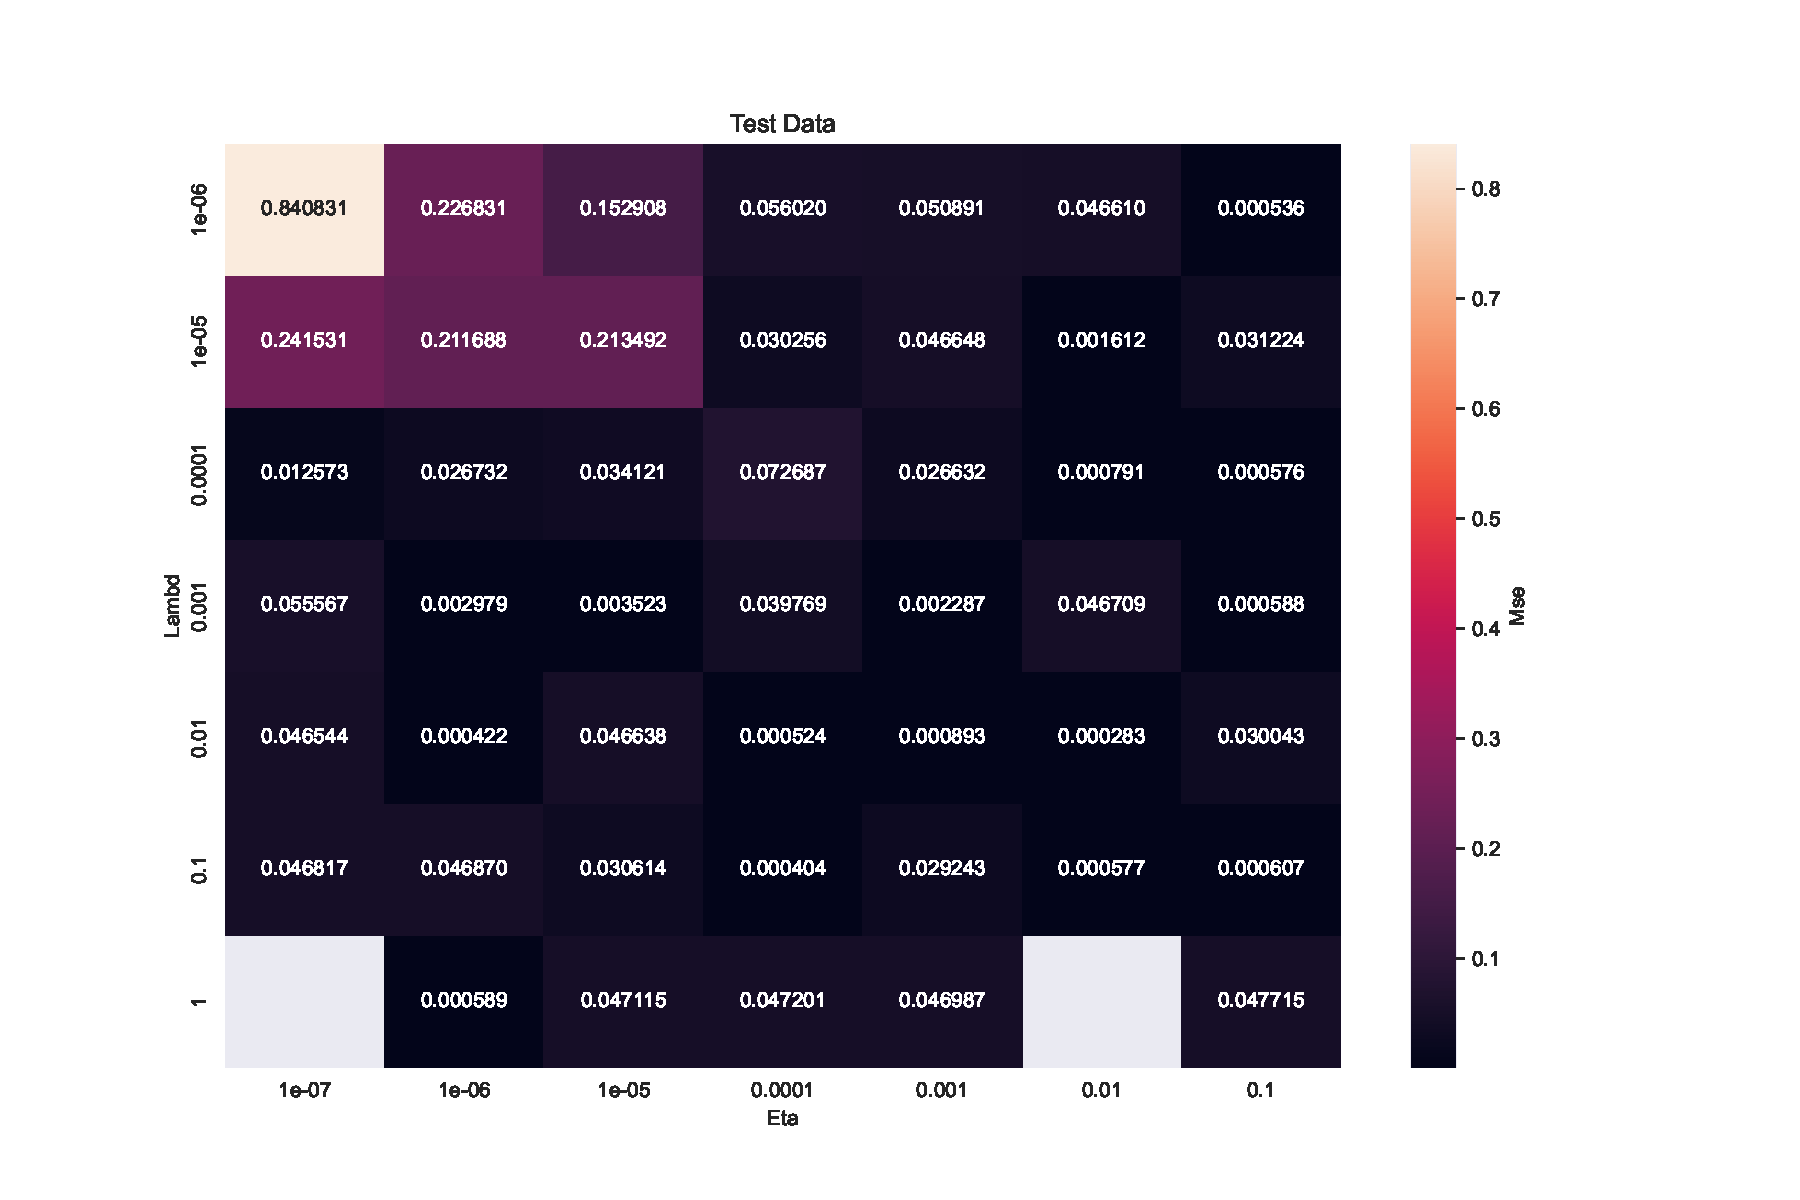
\includegraphics[width=1.2\linewidth]{Figures/PartB/test_leaky_relu_MSE(eta,lmb)}
  \caption{Test MSE}
  \label{fig:test_leaky_relu_MSE-eta-lmb-}
\end{subfigure}
\caption{Neural network with activation function leaky relu MSE as a function of \(\eta \) and \(\lambda \) }
\label{fig:leaky_relu_MSE}
\end{figure}


